% JHEP format. The style package jheppub supplies the page layout, natbib,
% hyperref and the \abstract macro; the bibliography style JHEP.bst is selected
% at the end of this file. amsmath, amssymb, graphicx are loaded by jheppub.
\documentclass[11pt,a4paper]{article}
\usepackage{jheppub}
\usepackage[T1]{fontenc}
\usepackage{bm}
\usepackage{booktabs}
\usepackage{array}
\usepackage{tikz}
\usetikzlibrary{arrows.meta}
\usetikzlibrary{shapes.geometric}

\setlength{\emergencystretch}{2em}
\sloppy

\newcommand{\dd}{\mathrm d}
\newcommand{\ii}{\mathrm i}
\newcommand{\Id}{\mathbb I}
\newcommand{\diag}{\operatorname{diag}}

\title{\bf FlintNDE: a FLINT-based package for high-precision numerical
solution of matrix differential equations}

\author[a,b]{Jiaqi Chen}
\affiliation[a]{Beijing Key Laboratory of Optical Detection Technology for Oil and Gas,
China University of Petroleum-Beijing, Beijing 102249, China}
\affiliation[b]{Basic Research Center for Energy Interdisciplinary, College of Science,
China University of Petroleum-Beijing, Beijing 102249, China}
\emailAdd{jiaqichen@cup.edu.cn}

\abstract{
First-order matrix differential equations with rational coefficient matrices form the
shared numerical core of three lines of calculation: dimensionally regularized Feynman
integrals in flat-spacetime quantum field theory, cosmological correlators in de Sitter
space obtained through the same integration-by-parts and differential-equation strategy,
and radial connection problems in black-hole perturbation theory. We present
\texttt{FlintNDE}, a
Python package that solves such systems along paths in the complex plane to user-specified
high precision. It is built on the FLINT library and performs all arithmetic in
midpoint-radius ball arithmetic, so that every returned value carries a rigorous error
estimate. Local solutions are generalized power series, that is, a power factor, powers of
a logarithm and a Taylor remainder. Wherever the input is exact, the underlying structure
(singularity locations, indicial spectrum, logarithm degrees) is certified in exact
Gaussian-rational arithmetic. As one further capability, decoupled essential singularities,
where the high-order pole part splits into scalar sectors, are handled with certified
exponential-polynomial phases. The package plans paths adaptively around the certified
singularities, separates planning from execution, records reusable save points, reconstructs
Laurent series in an analytic regulator following the sampling procedure of AMFlow, and
evaluates batches of regulator values in parallel. A Wolfram Language
interface exposes the same functionality. We demonstrate all eight shipped examples,
including the two-ended connection problem for the $\ell=2$ Schwarzschild quasinormal mode,
and verify the results against independent references.
}

\begin{document}
\maketitle

\section{Introduction}
\label{sec:introduction}

High-precision numerical evaluation is now a standard step in three families of physics
calculations. In flat-spacetime quantum field theory, multi-loop Feynman integrals enter
cross sections for collider processes and are reduced to master integrals by
integration-by-parts (IBP) relations \cite{Chetyrkin:1981qh}, whose induced differential equations (DE)
\cite{Kotikov:1990kg,Kotikov:1991pm,Bern:1993kr,Gehrmann:1999as}, often brought to the
canonical d log form \cite{Henn:2013pwa}, are then
solved from boundary data. In de Sitter (dS) space, late-time correlation functions connect
the dynamics of fields during inflation to the statistical properties of primordial
fluctuations \cite{Chen:2017ryl,Arkani-Hamed:2018kmz,Xianyu:2023ytd}, and the same
IBP-to-DE strategy has recently been extended to their time integrals
\cite{Chen:2023iix,Chen:2024glu,Chen:2026dqp}. In black-hole physics, the linear
perturbations of the Schwarzschild geometry separate into radial Regge--Wheeler and Zerilli
equations \cite{Regge:1957td,Zerilli:1970se}, and their quasinormal modes (QNM)---the
ringdown signals observed in gravitational-wave detections
\cite{LIGOScientific:2016aoc}---are defined by a two-ended boundary-value problem
\cite{Leaver:1985ax,Berti:2009kk}. All three settings reduce, after symbolic preparation,
to the same numerical object: a first-order system
$\dd Y/\dd z=A(z)\,Y$ with rational or analytic coefficient matrix, to be transported
reliably between points of the complex plane.

A mature toolbox exists on the symbolic side. FIRE \cite{Smirnov:2019qkx,Smirnov:2025prc},
Kira \cite{Maierhofer:2017gsa,Klappert:2020nbg,Lange:2025fba} and AmpRed
\cite{Chen:2024xwt} generate IBP reductions; expansion by regions
\cite{Beneke:1997zp,Pak:2010pt} and dimensional recurrence \cite{Lee:2010wea} provide
complementary asymptotic information. On the numerical side, DiffExp
\cite{Hidding:2020ytt} transports solutions along piecewise-linear paths in terms of
one-dimensional series expansions, and the auxiliary mass flow method of AMFlow
\cite{Liu:2017jxz,Liu:2020kpc,Liu:2022chg} solves the DE at a sequence of auxiliary mass
values and reconstructs the Laurent series in the dimensional regulator. Both are
Mathematica packages. The recent AMFlow 2.0 release additionally provides a
high-performance differential-equation solver written in C$^{++}$, connected to Mathematica
through WSTP and also available as a standalone, configuration-driven command-line
executable that reads the differential-equation matrix and the boundary values from plain
input files \cite{Huang:2026rjb}. Along the path, the local series that both methods
transport are generalized power series---a power factor, powers of a logarithm, and a
Taylor remainder---as introduced for Feynman-integral differential equations in
ref.~\cite{Moriello:2019yhu}.

\texttt{FlintNDE} is a plain, fast numerical solver for exactly this class of systems,
implemented in Python on top of the FLINT library \cite{Johansson:2017arb,PythonFlint}. It
takes an already-reduced matrix differential equation together with certified boundary data
and returns values, local series and Laurent coefficients to user-specified precision; it
does not generate IBP relations and does not manage integral families. Where the
\texttt{desolver} executable packages the AMFlow differential-equation module for users who
want it without the rest of the pipeline, \texttt{FlintNDE} additionally provides, for the
same class of systems, explicit path planning with singularity avoidance and jumps, coverage
of dense sets of requested points by shared series coefficients
(section~\ref{sec:efficiency}), and certified exponential-polynomial phases at decoupled
essential singularities (section~\ref{sec:high-order}). Its design choices are the
following.
\begin{enumerate}
\item All floating-point arithmetic uses Arb ball numbers \cite{Johansson:2017arb}: every
returned component carries a radius, and the default working precision is 200 decimal
digits. Interval results, not point estimates, decide whether a requested relative error
has been met.
\item Whenever the input matrix is exact over Gaussian rationals, the structural decisions
are made in exact arithmetic: singularities are discovered from the matrix entries, the
matrix indicial equation is solved over $\mathbb Q(\ii)$, and logarithm degrees follow from
Jordan structure and resonance conditions. Where a
 certified structure is required but unavailable, the package reports failure instead of
 silently degrading.
\item Local solutions are the generalized power series of ref.~\cite{Moriello:2019yhu}.
As one additional capability, decoupled essential singularities, whose high-order pole
part splits into scalar sectors, are handled by exact exponential-polynomial phases, and a
start-only formal asymptotic branch exists for second-order poles with simple distinct
leading spectrum; no systematic treatment of general high-order poles is attempted.
\item Path planning is separated from execution. Plans serialize with their precision, avoid
certified singularities by default, and can be executed only at or below the planning
precision. Explicit singularity jumps and strictly user-supplied node chains are available
options.
\item Laurent reconstruction in an analytic regulator reuses the complete numerical
transport at exact rational regulator values and follows the empirical sampling plan of
AMFlow 2.0 \cite{Huang:2026rjb}, with an explicit candidate-pool semantics and independent
validation points.
\item The same functionality is exposed through a Wolfram Language interface, and batches
of fixed regulator values can be evaluated in a bounded process pool.
\end{enumerate}

The package is used as the numerical backend of the \texttt{MadStree} package for dS tree
correlators, where it transports d log-form systems and reconstructs regulator series, and
independently for black-hole radial problems. Sections~\ref{sec:contract} and
\ref{sec:transport}--\ref{sec:reconstruction} specify the mathematical object, the
transport engine and the regulator reconstruction. Section~\ref{sec:usage} describes usage
from Python and from Wolfram Language. Section~\ref{sec:examples} presents the eight
shipped examples, including the Schwarzschild QNM connection problem, and
section~\ref{sec:verification} reports verification against independent references.

\section{The problem and the interface contract}
\label{sec:contract}

\subsection{Systems and input formats}
\label{sec:systems}

We consider column-vector systems
\begin{equation}
  \frac{\dd}{\dd z}Y(z)=A(z)\,Y(z),
  \qquad A(z)\in\mathbb C^{N\times N},
  \label{eq:matrix-system}
\end{equation}
where $A(z)$ is either an exact matrix of rational functions over $\mathbb Q(\ii)$ or an
arbitrary analytic callable. The exact class is entered as coefficient records with
constant term first,
\begin{equation}
  A_{ij}(z)=\frac{p_{ij}(z)}{q_{ij}(z)},\qquad
  p_{ij},\,q_{ij}\in\mathbb Q(\ii)[z],
  \label{eq:rational-entries}
\end{equation}
and every coefficient accepts integers, fractions, decimal strings or
\texttt{"a+b*I"} records. Floating-point input is rejected on the exact route: raising the
working precision cannot recover input digits that were never there.

For exact input, finite singularities, their pole orders and the classification of infinity
are discovered internally from the denominators; the user supplies neither pole positions
nor residues. The solver also recognizes the special structure
\begin{equation}
  A(x)=P(x)+\sum_j\frac{R_j}{x-p_j},
  \label{eq:polynomial-simple-poles}
\end{equation}
where $P(x)$ is a matrix polynomial of arbitrary finite degree; an explicitly known
decomposition of this form may be supplied directly, which is an optimization, not a
requirement. General rational matrices and analytic callables use the generic route, and
pure polynomial systems form the legal special case of an empty pole set.
Section~\ref{sec:efficiency} describes when the transport verifies
identity~\eqref{eq:polynomial-simple-poles} internally and switches to a fast recurrence
route.

\subsection{Local solutions as generalized power series}
\label{sec:local-solutions}

At an ordinary point $c$, write $s=z-c$ and expand $A(c+s)=\sum_{m\ge0}A_m(c)s^m$. The
solution coefficients obey the triangular recurrence
\begin{equation}
  Y_{n+1}(c)=\frac{1}{n+1}\sum_{m=0}^{n}A_m(c)\,Y_{n-m}(c).
  \label{eq:ordinary-recurrence}
\end{equation}
The matrix Taylor coefficients $A_m(c)$ are recovered numerically by Cauchy
sampling---evaluations on a circle followed by a discrete Fourier projection---which
requires only analyticity inside the sampling disc.

At a regular singular point, a Fuchsian system
$\dd Y/\dd z=(R/z+\sum_{m\ge0}A_mz^m)Y$ has local solutions
\begin{equation}
  Y=z^\rho\sum_{n\ge0}\sum_{q=0}^{q_{\max}}v_{n,q}\,z^n(\log z)^q,
  \label{eq:power-log-form}
\end{equation}
where the exponents $\rho$ solve the matrix indicial equation
\begin{equation}
  \det(\rho\Id-R)=0,
  \label{eq:matrix-indicial}
\end{equation}
and the coefficients obey, at fixed $(n,q)$,
\begin{equation}
  \bigl((\rho+n)\Id-R\bigr)v_{n,q}+(q+1)\,v_{n,q+1}
  =\sum_{m=0}^{n-1}A_m\,v_{n-1-m,q}.
  \label{eq:power-log-recurrence}
\end{equation}
Two distinct mechanisms produce logarithms. A Jordan block of length $\nu$ in $R$ gives
$z^\rho\sum_{q<\nu}(N^q/q!)(\log z)^q$ with $N=R-\rho\Id$. Even for a diagonalizable
residue, equation~\eqref{eq:power-log-recurrence} becomes singular when $\rho+n$ is
another indicial root: a pure-power recurrence survives only if the spectral projector
compatibility $P_{\rho+n}b_n=0$ holds, and the defect otherwise migrates into a
logarithmic coefficient. The package decides both mechanisms in exact rational arithmetic.

Boundary data at a singular start are therefore specified as leading branches
\begin{equation}
  \{a,\;b,\;C\}\;:\qquad Y(z)\sim z^{a}(\log z)^{b}\,C+\cdots,
  \label{eq:frobenius-boundary-record}
\end{equation}
with $a$ and the components of $C$ exact over $\mathbb Q(\ii)$, $b$ a non-negative integer
and $C$ of the system dimension; several records may be superposed. For example, the
branch $3x^{2}$ of $\dd y/\dd x=2y/x$ is entered as $\{a{=}2,\,b{=}0,\,C{=}[3]\}$. The
vector $C$ must lie
in the certified eigenspace (or, for a Jordan branch, satisfy $NC=0$ and lie in the image
of $N^b$); lower logarithmic degrees of a Jordan chain are completed automatically from
$\exp(N\log z)$.

At a decoupled essential singularity, all Laurent matrices of pole order two and higher
are simultaneously diagonal in the eigenbasis of the leading one, and lower-order terms
do not couple sectors with different exponential signatures. The scalar high-order part
$\sum_{m\ge2}c_mz^{-m}\Id$ is then removed by
\begin{equation}
  Y=e^{\Phi(z)}\,U,\qquad
  \Phi(z)=-\sum_{m=2}^{p}\frac{c_m}{m-1}\,z^{-(m-1)},
  \label{eq:implemented-exponential-factor}
\end{equation}
after which the residual system must have pole order at most one and the power--log
machinery of equation~\eqref{eq:power-log-recurrence} applies to $U$. The corresponding
boundary records extend to
\begin{equation}
  \{\phi,\;a,\;b,\;C\}\;:\qquad Y(z)\sim e^{\phi(z)}\,z^{a}(\log z)^{b}\,C+\cdots,
  \label{eq:exponential-boundary-record}
\end{equation}
where the phase $\phi$ lists the coefficients of the negative powers of the local
variable, with exact values derived from the differential equation and verified entry by
entry; for $\dd y/\dd x=y/x^{2}$, whose solutions are $C\,e^{-1/x}$, it is the single term
$\phi=\{-1\mapsto-1\}$. This
extends the generalized power series of ref.~\cite{Moriello:2019yhu} beyond the
logarithmic structure for this certified class of singularities.

\subsection{Scope}
\label{sec:scope}

The package consumes matrix differential equations and boundary data; it does not generate
IBP relations, does not read integral families, master orderings or normalizations, and
does not infer the Laurent support of a regulator expansion from numerical samples---the
lowest Laurent power must be certified upstream. Structures that would require
ramified formal gauges, algebraic field extensions beyond $\mathbb Q(\ii)$, general formal
block decoupling or Stokes connection matrices are not implemented; whenever the certified
route to a requested local basis does not exist, the package raises an exception rather
than returning an uncertified value. Section~\ref{sec:high-order} delimits the irregular
case precisely.

\section{Core function I: numerical transport}
\label{sec:transport}

\subsection{Overview}
\label{sec:overview}

A calculation proceeds in five stages. First, the exact system is analyzed and a
singularity inventory is produced: locations, pole orders, and the classification of each
point as ordinary, regular singular or irregular, including the point at
infinity. Second, local solution bases are constructed at the requested endpoints. Third,
a path is planned in the complex plane, with planning separated from execution
(section~\ref{sec:paths}). Fourth, the solution is transported segment by segment: each
segment carries the Taylor recurrence of equation~\eqref{eq:ordinary-recurrence} inside a
Cauchy disc that contains no singularity. Fifth, results are written as save points
together with a summary, and a two-chain error estimate is returned
(sections~\ref{sec:paths} and~\ref{sec:error-control}). Figure~\ref{fig:transport-workflow}
summarizes the pipeline.

\begin{figure}[p]
\centering
\scriptsize
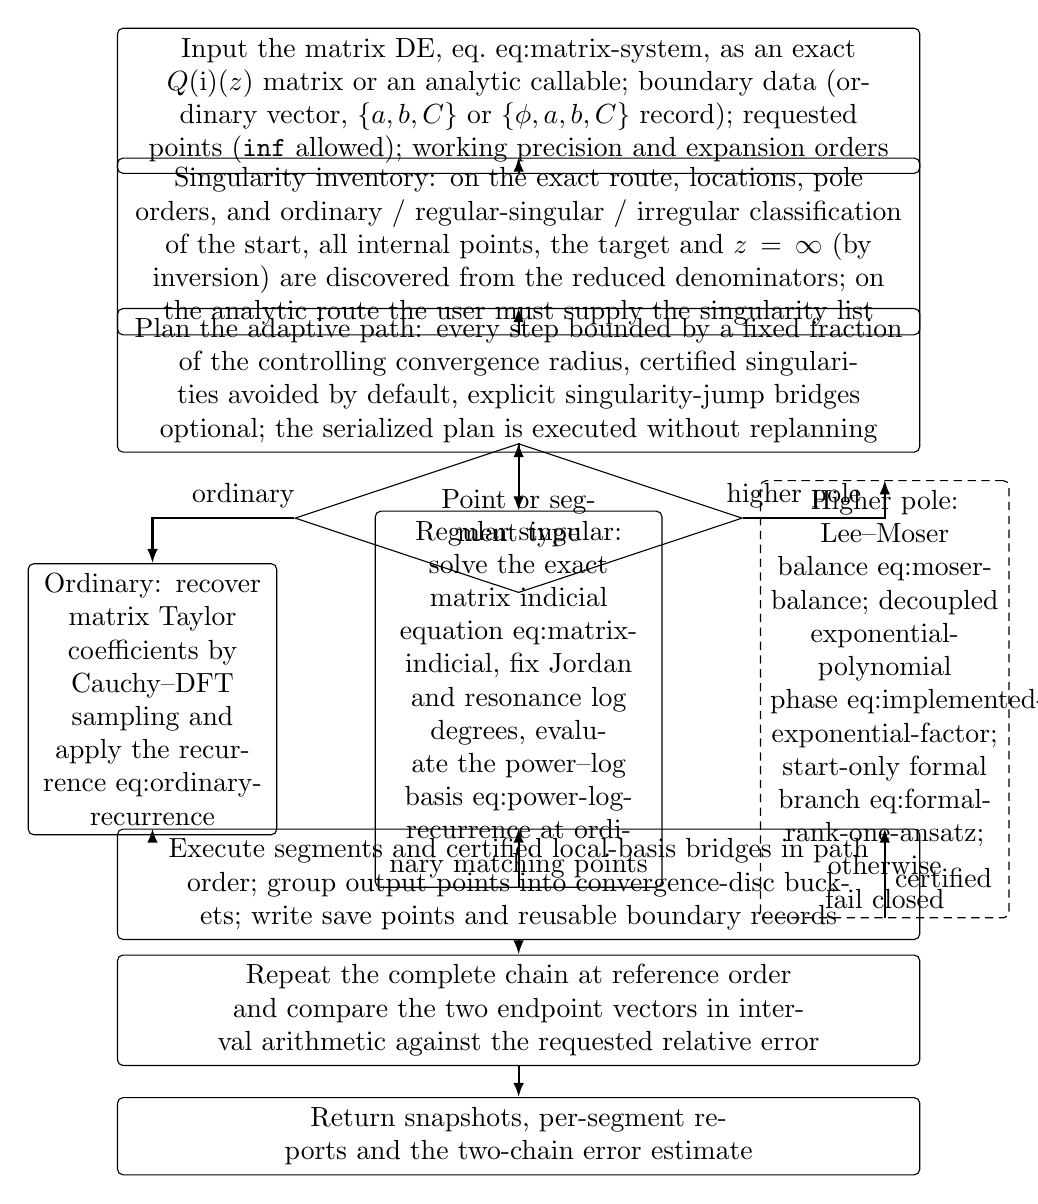
\begin{tikzpicture}[
  box/.style={draw, rounded corners=2pt, align=center, inner sep=3.5pt},
  decision/.style={draw, diamond, aspect=3.0, align=center, inner sep=1.2pt},
  flow/.style={-{Latex[length=1.8mm]}, thick},
  fail/.style={draw, rounded corners=2pt, align=center, inner sep=3.5pt, densely dashed}
]
\node[box, text width=.82\textwidth] (input) at (0,0)
  {Input the matrix DE, eq.~\eqref{eq:matrix-system}, as an exact
   $\mathbb Q(\ii)(z)$ matrix or an analytic callable; boundary data (ordinary vector,
   $\{a,b,C\}$ or $\{\phi,a,b,C\}$ record); requested points (\texttt{inf} allowed);
   working precision and expansion orders};
\node[box, text width=.82\textwidth] (inventory) at (0,-1.85)
  {Singularity inventory: on the exact route, locations, pole orders, and ordinary /
   regular-singular / irregular classification of the start, all internal points, the
   target and $z=\infty$ (by inversion) are discovered from the reduced denominators; on
   the analytic route the user must supply the singularity list};
\node[box, text width=.82\textwidth] (path) at (0,-3.55)
  {Plan the adaptive path: every step bounded by a fixed fraction of the controlling
   convergence radius, certified singularities avoided by default, explicit
   singularity-jump bridges optional; the serialized plan is executed without replanning};
\node[decision, text width=.26\textwidth] (kind) at (0,-5.30)
  {Point or segment type};
\node[box, text width=.24\textwidth] (ordinary) at (-4.65,-7.60)
  {Ordinary: recover matrix Taylor coefficients by Cauchy--DFT sampling and apply the
   recurrence~\eqref{eq:ordinary-recurrence}};
\node[box, text width=.28\textwidth] (regular) at (0,-7.60)
  {Regular singular: solve the exact matrix indicial
   equation~\eqref{eq:matrix-indicial}, fix Jordan and resonance log degrees, evaluate the
   power--log basis~\eqref{eq:power-log-recurrence} at ordinary matching points};
\node[fail, text width=.24\textwidth] (irregular) at (4.65,-7.60)
  {Higher pole: Lee--Moser balance~\eqref{eq:moser-balance}; decoupled
   exponential-polynomial phase~\eqref{eq:implemented-exponential-factor}; start-only
   formal branch~\eqref{eq:formal-rank-one-ansatz}; otherwise fail closed};
\node[box, text width=.82\textwidth] (transport) at (0,-9.95)
  {Execute segments and certified local-basis bridges in path order; group output points
   into convergence-disc buckets; write save points and reusable boundary records};
\node[box, text width=.82\textwidth] (refine) at (0,-11.55)
  {Repeat the complete chain at reference order and compare the two endpoint vectors in
   interval arithmetic against the requested relative error};
\node[box, text width=.82\textwidth] (output) at (0,-13.15)
  {Return snapshots, per-segment reports and the two-chain error estimate};

\draw[flow] (input) -- (inventory);
\draw[flow] (inventory) -- (path);
\draw[flow] (path) -- (kind);
\draw[flow] (kind) -| node[pos=.18,above]{ordinary} (ordinary.north);
\draw[flow] (kind) -- (regular);
\draw[flow] (kind) -| node[pos=.18,above]{higher pole} (irregular.north);
\draw[flow] (ordinary.south) -- (ordinary.south |- transport.north);
\draw[flow] (regular) -- (transport);
\draw[flow] (irregular.south) -- node[pos=.45,right]{certified} (irregular.south |- transport.north);
\draw[flow] (transport) -- (refine);
\draw[flow] (refine) -- (output);
\end{tikzpicture}
\caption{The numerical transport pipeline. Input formats and the scope contract are given in
section~\ref{sec:contract}; local solution structures in section~\ref{sec:local-solutions};
exact certification and the floating-point route in section~\ref{sec:certification}; the
three higher-pole routes and their fail-closed boundary in section~\ref{sec:high-order};
path planning, singularity jumps and save points in section~\ref{sec:paths}; efficiency
features in section~\ref{sec:efficiency}; and two-chain error control in
section~\ref{sec:error-control}.}
\label{fig:transport-workflow}
\end{figure}

\subsection{Exact structure certification and the numerical route}
\label{sec:certification}

For exact input, the indicial roots, Jordan nilpotency, spectral projectors and every
active resonance gate are determined by FLINT rational matrices and stored in a manifest;
FLINT then evaluates equation~\eqref{eq:power-log-recurrence} at the requested precision.
An exact failure never falls back to a threshold decision.

When the original input is floating-point data, an explicit numerical route exists. It
classifies the structure with a relative cutoff scaled by the system dimension and by the
reliable decimal precision of the input---Python binary64 input is capped at 15 digits
regardless of the working precision, and higher-precision input must declare its reliable
precision. Every numerical classification emits a warning and a manifest recording the
matrix scale, both cutoffs, and the largest zeroed and smallest retained quantities;
ambiguous mixed-root defective systems fail closed. The exact cutoff formula is given in
appendix~\ref{app:exact}.

\subsection{High-order poles}
\label{sec:high-order}

A pole of order $p\ge2$ in some matrix entry triggers a three-route dispatch.
First, an exact Lee--Moser projector balance is attempted: from the top two Laurent
matrices a projector $Q$ with $Q^2=Q$ is constructed and the gauge transformation
\begin{equation}
  I=\Bigl(1-Q+\frac{Q}{z}\Bigr)J
  \label{eq:moser-balance}
\end{equation}
is applied; each round must lower the pole order strictly, and the complete transformed
system is verified by an exact round trip. Success reduces the point to the power--log
case, with the boundary transformed back to the original basis.

If a high-order pole remains, the second route applies at decoupled essential
singularities as defined in section~\ref{sec:local-solutions}: the solution is the
exponential factor of equation~\eqref{eq:implemented-exponential-factor} times
a convergent power--log series. The third route applies when the pole order is exactly two
and the leading matrix has simple distinct eigenvalues $k_j$ over $\mathbb Q(\ii)$: for
each eigendirection it constructs the formal branch
\begin{equation}
  Y=e^{-k/z}\,z^{\rho}\sum_{n=0}^{N_{\rm form}}v_nz^n,
  \qquad \rho=\frac{\ell^{T}A_{-1}v_0}{\ell^{T}v_0},
  \label{eq:formal-rank-one-ansatz}
\end{equation}
with an exact recurrence for the $v_n$. This is a sectorial asymptotic series, not a
convergent Frobenius disk; it may only initialize a path start, and the package reports a
five-order block ratio and relative refinement
\begin{equation}
  r_5=\frac{\left\|\sum_{j=1}^{5}T_{N+j}\right\|_\infty}
  {\left\|\sum_{j=0}^{4}T_{N-j}\right\|_\infty},
  \qquad
  \delta_5=\frac{\|S_{N+5}-S_N\|_\infty}{\|S_{N+5}\|_\infty}
  \label{eq:formal-five-order-test}
\end{equation}
with $T_n=v_nz^n$, together with the least-term degree actually reached. The first
ordinary matching point is proposed from the exponential root gaps,
$|z|=\min_i\Delta_i/(qN)$ with $\Delta_i=\min_{j\ne i}|k_i-k_j|$ and default safety
factor $q=3$. All three routes fail closed on unsupported structure---defective leading
matrices, spectra outside $\mathbb Q(\ii)$, residual high-order poles after the scalar
extraction---with messages naming the missing reduction.

\subsection{Paths, singularities and transport}
\label{sec:paths}

Endpoints are named points; the literal string \texttt{"inf"} denotes infinity, which is
mapped to the zero of the inverted variable $\mathrm{sinv}=1/z$ with transformed matrix
$-\mathrm{sinv}^{-2}A(1/\mathrm{sinv})$. Paths are generated adaptively: each step is
bounded by a configurable fraction (default $0.45$) of the controlling convergence radius,
which is the distance to the nearest singularity whenever one exists. Planning and
execution are strictly separated: \texttt{FlintNDE} (Python entry
\texttt{plan\_transport\_path}) produces a complete serialized plan---including node
geometry with ball midpoints and radii and the planning precision---and execution
(\texttt{transport\_planned\_path\_refined}) restores and executes it without replanning;
on the Wolfram route, an execution requesting higher precision than the plan is rejected
and must be replanned.

By default the planner avoids certified singularities and returns structured diagnostics
when a straight segment hits one. The user may supply ordinary detour points, or enable
explicit singularity jumps, in which case the internal singularity is represented by a
local basis bridge between ordinary matching points rotated off the segment; the selected
multivalued branch is equivalent to some detour path and the winding numbers are reported,
since the responsibility for the branch choice stays with the user. A strict user-node
chain (\texttt{direct\_user\_point\_path}) disables planning entirely: no points are
inserted or removed, and hitting a singularity fails. A separate interface evaluates a
user-requested point that coincides with a finite singularity: removable components
return values, while genuine pole and logarithmically divergent components return the
classification text \texttt{Infinity} together with per-component orders.

Requested output points may carry a \texttt{"save"} tag. Save points are written
immediately as they are reached---ordinary points as vectors, singular points as reusable
$\{a,b,C\}$ or $\{\phi,a,b,C\}$ boundary records---and a failure later in the path leaves
the completed files intact and suppresses the summary.

\subsection{Efficiency}
\label{sec:efficiency}

Four features keep the solver fast without affecting the certified semantics.
\begin{enumerate}
\item \emph{Certified simple-pole recurrence.} Once
equation~\eqref{eq:polynomial-simple-poles} is verified exactly---by partial-fraction
decomposition of every entry, reconstruction of the right-hand side in
$\mathbb Q(\ii)(x)$, and independent ball-arithmetic probes at four sample
points---segment transport no longer performs Cauchy sampling: the polynomial part is
shifted by a binomial formula and
each pole contributes a geometric-series state $u_j[n]=(c[n]-u_j[n-1])/(c-p_j)$, one step
per Taylor coefficient, with residues read directly from the Laurent expansion.
\item \emph{Lookahead node selection and fast multipoint evaluation.} While planning, the
walker scans the remaining requested points in path order and places the next node at the
farthest requested point that, together with every intermediate point, still lies within
$0.9\,\kappa R$ of the current node, where $R$ is the distance to the nearest certified
singularity and $\kappa=\min(\kappa_{\rm user},1/4)$ caps the step fraction. The points it
steps over are not transported again: they become interior evaluation samples that share
the node's Taylor coefficients, so dense sets of requested points are covered by far fewer
transport steps. Samples of one segment form a bucket; buckets of eight or more points are
evaluated by the subproduct-tree algorithm of \texttt{acb\_poly}, smaller ones by
iterative evaluation. The algorithm actually used is recorded per bucket.
\item \emph{Batched singular starts.} Several Frobenius boundary vectors of one system
share the local basis and the per-segment Taylor matrices; only the column-wise error
gates are computed separately.
\item \emph{Process-level parallelism.} Because the FLINT precision context is
process-global, batches of independent fixed-regulator tasks run in a bounded spawn pool
(default twelve workers) instead of threads.
\end{enumerate}

\subsection{Error control}
\label{sec:error-control}

Every transport runs two chains: the primary chain at the production order produces all
user-visible values, and the reference chain at a higher order serves only for
certification; their relative difference at the final endpoint is compared against the
requested target, in interval arithmetic, and evaluated singular targets are certified
separately. Alternatively, an embedded certification mode reuses the leading prefix of a
single higher-order solve and reports the per-segment truncation differences. For formal
asymptotic branches, the five-order diagnostics of
equation~\eqref{eq:formal-five-order-test} are reported. These residuals are error
estimates, not rigorous bounds on the final error, and the returned status fields must be
inspected.

\section{Core function II: regulator-series reconstruction}
\label{sec:reconstruction}

\subsection{Problem and certificate}
\label{sec:reconstruction-problem}

Dimensionally regularized quantities take the form
$F(\varepsilon)=\sum_{n=n_{\min}}^{n_{\max}}f_n\varepsilon^n+O(\varepsilon^{n_{\max}+1})$.
Instead of truncating every intermediate expression in $\varepsilon$, the complete
numerical problem is solved at several small exact rational values $\varepsilon_j$ and the
coefficients are reconstructed; this is the strategy of AMFlow \cite{Liu:2022chg}. A finite
set of numerical solves cannot prove the Laurent support of a general callable, so the
interface requires the integer $n_{\min}$ together with a strict upstream certificate
(status, consistent integer, and method identification); missing or inconsistent
certificates fail before any solve. In the \texttt{MadStree} workflow the certificate is
generated automatically from the symbolic boundary and d log-form DE, while
\texttt{FlintNDE} itself remains independent of those data structures.
Figure~\ref{fig:reconstruction-workflow} summarizes the workflow; every regulator sample
invokes the complete transport pipeline of figure~\ref{fig:transport-workflow}.

\begin{figure}[t]
\centering
\footnotesize
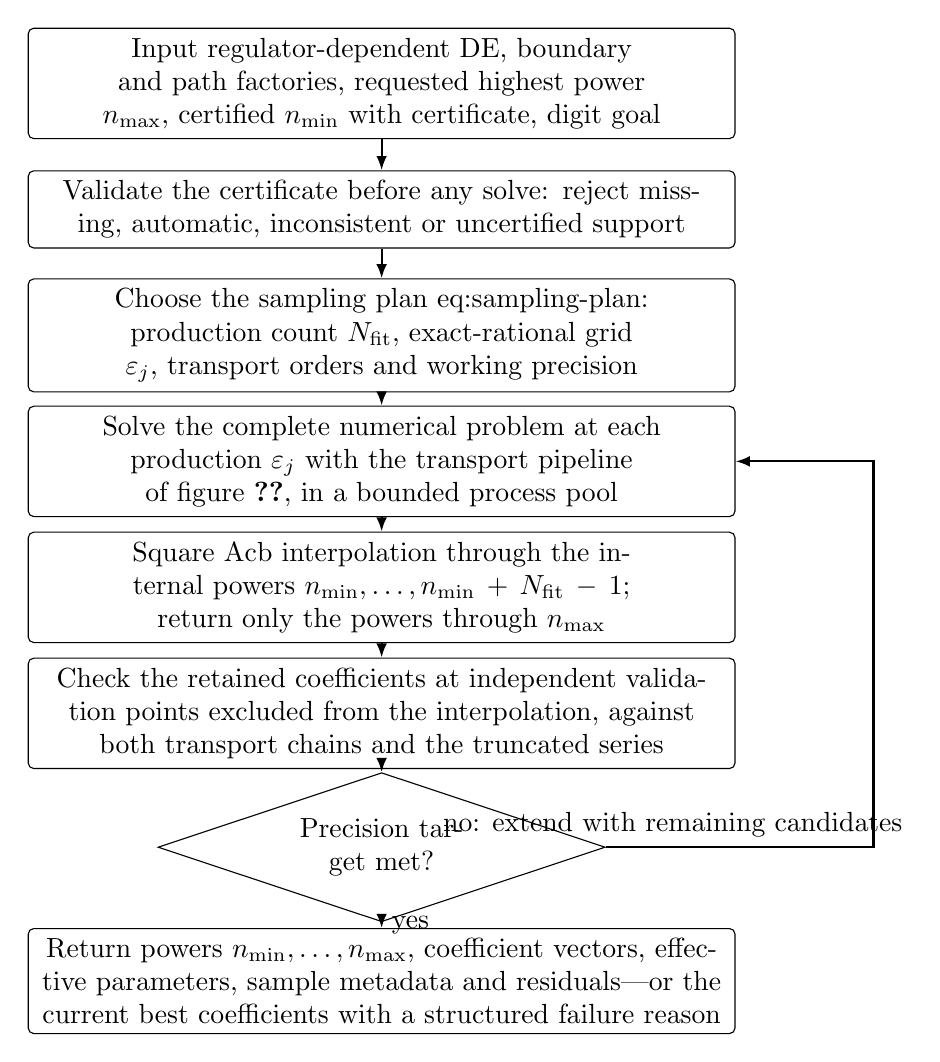
\begin{tikzpicture}[
  box/.style={draw, rounded corners=2pt, align=center, inner sep=3.5pt},
  decision/.style={draw, diamond, aspect=3.0, align=center, inner sep=1.2pt},
  flow/.style={-{Latex[length=1.8mm]}, thick},
  fail/.style={draw, rounded corners=2pt, align=center, inner sep=3.5pt, densely dashed}
]
\node[box, text width=.72\textwidth] (input) at (0,0)
  {Input regulator-dependent DE, boundary and path factories, requested highest power
   $n_{\max}$, certified $n_{\min}$ with certificate, digit goal};
\node[box, text width=.72\textwidth] (gate) at (0,-1.60)
  {Validate the certificate before any solve: reject missing, automatic, inconsistent or
   uncertified support};
\node[box, text width=.72\textwidth] (plan) at (0,-3.20)
  {Choose the sampling plan~\eqref{eq:sampling-plan}: production count $N_{\rm fit}$,
   exact-rational grid $\varepsilon_j$, transport orders and working precision};
\node[box, text width=.72\textwidth] (solve) at (0,-4.80)
  {Solve the complete numerical problem at each production $\varepsilon_j$ with the
   transport pipeline of figure~\ref{fig:transport-workflow}, in a bounded process pool};
\node[box, text width=.72\textwidth] (fit) at (0,-6.40)
  {Square Acb interpolation through the internal powers
   $n_{\min},\ldots,n_{\min}+N_{\rm fit}-1$; return only the powers through $n_{\max}$};
\node[box, text width=.72\textwidth] (validate) at (0,-8.00)
  {Check the retained coefficients at independent validation points excluded from the
   interpolation, against both transport chains and the truncated series};
\node[decision, text width=.26\textwidth] (met) at (0,-9.70)
  {Precision target met?};
\node[box, text width=.72\textwidth] (output) at (0,-11.40)
  {Return powers $n_{\min},\ldots,n_{\max}$, coefficient vectors, effective parameters,
   sample metadata and residuals---or the current best coefficients with a structured
   failure reason};

\draw[flow] (input) -- (gate);
\draw[flow] (gate) -- (plan);
\draw[flow] (plan) -- (solve);
\draw[flow] (solve) -- (fit);
\draw[flow] (fit) -- (validate);
\draw[flow] (validate) -- (met);
\draw[flow] (met) -- node[right]{yes} (output);
\draw[flow] (met.east) -- node[above,pos=.25]{no: extend with remaining candidates} ++(3.4,0) |- (solve.east);
\end{tikzpicture}
\caption{The regulator-series reconstruction workflow. Every production sample reuses the
complete transport pipeline of figure~\ref{fig:transport-workflow}; no separate
solution-fitting engine exists. The sampling formulas are discussed in
section~\ref{sec:sampling-plan} and the candidate-pool and validation semantics in
section~\ref{sec:pools}.}
\label{fig:reconstruction-workflow}
\end{figure}

\subsection{Sampling plan}
\label{sec:sampling-plan}

With $P=\max(0,-n_{\min})$ and $K=n_{\max}-n_{\min}$, the automatic plan follows the
empirical configuration of AMFlow 2.0 \cite{Huang:2026rjb} after the replacements
$2L\to P$ and $L/2\to P/4$ (the loop count $L$ is specific to the Feynman-integral pole
bound and is not a parameter of a general matrix system):
\begin{align}
  N_{\rm fit}&=\max\!\left(\left\lceil\tfrac52K+P\right\rceil,\,K+3\right),
  &\alpha_\varepsilon&=\tfrac P4+\frac{g}{K+1},\nonumber\\
  \varepsilon_0&\simeq10^{-\alpha_\varepsilon},
  &\varepsilon_j&=\varepsilon_0\,(1+j\,\delta),\quad j=1,\ldots,N_{\rm fit},
  \label{eq:sampling-plan}\\
  p_0&=\max\!\left(\left\lceil(N_{\rm fit}+P)\alpha_\varepsilon\right\rceil,\,30\right),
  &p_{\rm work}&=\max\!\left(200,\,\left\lceil2(1+p_{\rm extra})p_0\right\rceil\right).
  \nonumber
\end{align}
where $g$ is the digit goal, $\delta$ the relative sample spacing (default $0.01$), and
$p_0$ the transport-error goal in digits; the $K+3$ branch includes the default
\texttt{fit\_extra\_order}$\,=2$. The transport uses production order $4p_0$ and
reference order increased by $\lceil\max(50,p_0/5)\rceil$. The 200-digit floor is a
\texttt{FlintNDE} default; explicit user values override automatic planning.

All $N_{\rm fit}$ production samples enter a single square Acb Vandermonde solve for the
internal powers $n_{\min},\ldots,n_{\min}+N_{\rm fit}-1$; only coefficients through the
requested power $n_{\max}$ are returned, the extra powers absorbing truncation effects as
in the AMFlow construction. No least-squares or pseudo-inverse fit is used.

\subsection{Candidate pools, validation and complex sectors}
\label{sec:pools}

An explicit \texttt{sample\_points} sequence is an ordered production candidate pool: the
first round consumes only the prefix required by the current square system, and a failed
validation round consumes later candidates while reusing all previous solves. Once the
pool is exhausted, the package never invents regulator values outside the user-approved
range: it returns the current best coefficients with
\texttt{precision\_target\_met=False} and the structured reason
\texttt{candidate\_pool\_exhausted}. Independent validation points---by default on a
scaled production grid, or explicit and disjoint---never enter the interpolation and are
checked against both transport chains and the truncated series. Alternatively,
\texttt{sample\_angle\_range} restricts automatic complex sampling to an open angular
interval; at most three interior rays are selected, boundary rays are never used, and
radii continue to follow equation~\eqref{eq:sampling-plan}. A scalar fitting layer
(\texttt{fit\_sampled\_series}) reconstructs Laurent coefficients from samples the caller
has already computed, for quantities such as Wronskians that are not a single transport
endpoint.

\section{Using the package}
\label{sec:usage}

\subsection{Installation and loading}
\label{sec:installation}

The package requires Python $\ge3.10$ with \texttt{python-flint} $\ge0.6$ and
\texttt{sympy} $\ge1.12$, and installs from a wheel, from source, or in editable mode; on
first \texttt{import flintnde} it prints a one-line citation reminder to standard error
(suppressible through an environment variable, so that machine-readable standard output is
never polluted). Importing establishes the default 200-digit global precision;
\texttt{configure\_working\_precision(digits, guard)} resets it, with working bits
$\lceil \mathrm{digits}\cdot\log_2 10\rceil+32$. The Wolfram Language interface is loaded
by adding the package root to \texttt{\$Path} and calling \texttt{Needs["FlintNDE`"]}; it
launches the Python bridge with an argument-list \texttt{RunProcess}, writes bridge files
under a short-token directory, and reports its own error labels (for example
\texttt{PythonFlintUnavailable}, \texttt{BridgeLaunchFailed},
\texttt{RuntimePathTooLong}) when the runtime is misconfigured.

\subsection{Python interface: basic commands}
\label{sec:python-basic}

A calculation assembles an exact system, obtains the singularity inventory, plans a path,
and transports:
\begin{quote}\small
\begin{verbatim}
from flintnde import *
layout = initialize_output_layout(__file__, run_name="run01")
system = RationalMatrixSystem(entries, variable_name="s")
inventory = analyze_singularities(system, output_layout=layout)
path = build_adaptive_path(system, NamedPoint("start", 2),
                           NamedPoint("target", 3),
                           max_step_over_radius=0.45)
result = transport_path_refined(
    system, column_vector([1, 0]), path,
    primary_order=24, reference_order=32,
    target_relative_error="1e-15")
# result["primary_snapshots"], result["relative_difference_inf"], ...
\end{verbatim}
\end{quote}
Entries are built with \texttt{rational\_function}, whose numerator and denominator
coefficients accept all exact formats of section~\ref{sec:systems}; sums of rational
functions are merged and cancelled exactly before denominators are collected. Singular
starts use the boundary records of equations~\eqref{eq:frobenius-boundary-record}
and~\eqref{eq:exponential-boundary-record} through \texttt{frobenius\_boundary} and
\texttt{exponential\_boundary}, which validate the exponents and vectors against the exact
manifest before any transport. Save points are requested by appending the string
\texttt{"save"} to a coordinate, and a capability pre-check
(\texttt{build\_adaptive\_path\_plan}) classifies all endpoints and internal singularities
without numerical work, returning whether the requested continuation is certified.

\subsection{Python interface: reconstruction and parallel evaluation}
\label{sec:python-advanced}

The minimal reconstruction call passes the complete numerical problem, the highest
requested power, and the upstream certificate:
\begin{quote}\small
\begin{verbatim}
result = reconstruct_series_solution(
    DEmatrix=DEmatrix, boundary=boundary, path=path,
    maximum_power=2, leading_power=-1,
    leading_power_certificate={
        "status": "certified", "leading_power": -1,
        "method": "symbolic-boundary-and-DE"})
\end{verbatim}
\end{quote}
If the matrix, boundary or path depend on the regulator, they are passed as factories that
receive exact rational regulator values, keeping every automatically generated sample
exact. The result exposes \texttt{coefficient(power)}, \texttt{evaluate(ep)}, the
production and validation values, the effective parameters, and per-round diagnostics.
Independent fixed-regulator tasks run through \texttt{run\_ep\_tasks}, which starts at
most \texttt{parallel\_task\_count} (default 12) workers and hands the next task to
whichever worker finishes first.

\subsection{Wolfram Language interface}
\label{sec:wolfram}

The Wolfram interface mirrors the plan--execute separation of section~\ref{sec:paths}:
\begin{quote}\small
\begin{verbatim}
Needs["FlintNDE`"];
system = FlintNDERationalSystem[{{1/(x - 1)}}, x];
plan   = FlintNDEPlanPath[system, 0, {1/2},
          "WorkingPrecisionDigits" -> 100,
          FlintNDE`SingularityMode -> "Avoid"];
result = FlintNDEExecutePath[system, {1}, plan,
          "PrimaryOrder" -> 40, "ReferenceOrder" -> 48,
          "TargetRelativeError" -> "1e-30"];
\end{verbatim}
\end{quote}
\texttt{FlintNDERationalSystem} accepts any exact rational matrix and discovers the
singularities internally; \texttt{FlintNDEPartialFractionSystem} constructs an explicitly
known decomposition of the form~\eqref{eq:polynomial-simple-poles}, which is an
optimization and never a requirement. \texttt{FlintNDEEvaluateEpBatch} evaluates a list of
fixed-regulator jobs with the option \texttt{ParallelTaskCount} (default 12) and returns
results in input order. Options control the working and output digits, the two transport
orders, the relative-error target, the singularity mode (\texttt{"Avoid"} or
\texttt{"SingularityJump"}), and the message language; \texttt{"WorkDirectory"} denotes
the temporary run root for bridge files. Errors surface as \texttt{Failure} objects with
the bridge labels of section~\ref{sec:installation}.

\subsection{Options and common pitfalls}
\label{sec:pitfalls}

Working precision is a global setting: \texttt{OutputDigits} formats output but never
raises internal precision. Executing a serialized plan above its planning precision is
rejected (section~\ref{sec:paths}). Exact routes reject
\texttt{float}/\texttt{complex} input; numerical structure classification requires a
declared reliable input precision. The batched singular-start entry accepts only paths
whose transitions are all ordinary Taylor segments and writes no save files; individual
calls to \texttt{transport\_path\_refined} cover those cases. Singularity-mode strings
differ between the interfaces (\texttt{"avoid"}/\texttt{"singularity\_jump"} in Python,
\texttt{"Avoid"}/\texttt{"SingularityJump"} in Wolfram), and messages are English by
default.

\section{Examples}
\label{sec:examples}

The package ships eight runnable examples. The numbers below were produced by fresh runs
of the released scripts with \texttt{python-flint} 0.9.0 on Python 3.12 and Wolfram
Language 15.0; the five examples that request output layouts leave JSON summaries under
their own \texttt{results/} directories.

\subsection{Scalar endpoints with save points}
\label{sec:example-saves}

Three scalar examples exercise the singular-boundary records.
The first, $\dd y/\dd x=2y/x$ with exact solution $3x^2$, starts at the regular singular
point $x=0$ from the branch $\{a{=}2,b{=}0,C{=}[3]\}$ and transports to $x=1$ at 50
working digits with primary and reference orders 20 and 28: the returned value is
$3.0000000000000000000000000000000000000000000000000000000$ with relative ball radius
$7.7\times10^{-57}$, and the primary/reference relative difference is zero. The second,
$\dd y/\dd x=y/x^{2}$ with solution $C\,e^{-1/x}$, starts at the decoupled irregular
singularity $x=0$ from the record $\{\phi{=}\{-1\!\mapsto\!-1\},a{=}0,b{=}0,C{=}[3]\}$:
at $x=1$ it returns
$3e^{-1}=1.1036383235143269649064597241584202227841610166983386677$ with a spurious
imaginary component of magnitude $7.9\times10^{-57}$ (ball radius $3.5\times10^{-114}$),
and the save file written at the singular
start can be re-read by \texttt{exponential\_boundary} to reconstruct the identical
boundary object.

The third scalar example exercises multi-term exponential phases at a third-order pole.
The diagonal system
\begin{equation}
  A(z)=\diag\!\left(\frac{3}{2z^{3}}+\frac{1}{z^{2}}+\frac{1}{2z}+2,\;
  \frac{1}{z^{3}}+\frac{1}{3z^{2}}+\frac{7}{2z}-1\right)
  \label{eq:exponential-polynomial-system}
\end{equation}
has at $z=0$ a decoupled essential singularity whose two sectors carry the polynomial
phases $\Phi_{1}=-3/(4z^{2})-1/z$ and $\Phi_{2}=-1/(2z^{2})-1/(3z)$ and the residual
powers $a=1/2$ and $a=7/2$; the boundary consists of two $\{\phi,a,b,C\}$ records, one per
sector, each phase containing two negative powers in contrast to the single term above.
The closed-form solution $(z^{1/2}e^{\Phi_{1}+2z},\;z^{7/2}e^{\Phi_{2}-z})$ equals
$(e^{1/4},\,e^{-11/6})$ at $z=1$; the transport with orders 48 and 64 and sampling
fraction 0.45 reproduces these values with relative differences $6.0\times10^{-25}$ and
$3.9\times10^{-25}$, meeting the requested $10^{-14}$ target, and saves both endpoints.

\subsection{Regulator Laurent-series reconstruction}
\label{sec:example-reconstruction}

The reconstruction example combines a zero connection (the boundary value is transported
unchanged) with the symbolic boundary
$1/\varepsilon+2+3\varepsilon+4\varepsilon^{2}+5\varepsilon^{3}+6\varepsilon^{4}$, so that
the certified leading power $-1$ and every coefficient are known. The user supplies seven
production candidates and two validation points, caps the first internal power at 2, and
requests 12 digits. The first round consumes only the four-point prefix; its independent
validation fails with relative residual $1.2\times10^{-4}$. The second round adds two
candidates---reusing all four previous production solves and both validation solves---and
passes with residual $5.7\times10^{-44}$, returning the pole coefficient 1 and the finite
part 2 to better than $10^{-30}$; one candidate remains unused. A second run with
\texttt{sample\_angle\_range}$\,=(-\pi/3,\pi/3)$ places all automatic samples on exactly
three interior rays inside the open sector and still certifies the digit goal.

\subsection{Wolfram Language interface walkthrough}
\label{sec:example-wolfram}

The interface example constructs the diagonal system
$A(z)=\diag(1/(z-1),-2/(z+3))$ with $Y(0)=(1,1)$, plans in \texttt{"Avoid"} mode at 80
working digits, and executes the plan without replanning. Evaluated at the target
$z=1/2$, the primary/reference relative
difference is $3.4\times10^{-45}$, the certification mode is reported as certified, and
the final vector agrees with the closed form $(1/2,\,36/49)$ through the first 39
digit at the requested 40 output digits.

\subsection{Parallel batches of fixed regulator values}
\label{sec:example-parallel}

The equation $\dd y/\dd x=\varepsilon\,y/(1+x)$ with $y(0)=1$ has the closed form
$y(1)=2^{\varepsilon}$. The Python entry evaluates $\varepsilon\in\{1/5,1/6,1/7\}$ in a
pool requested at twelve workers (three effective) at 60 working digits with orders 112
and 128; for $\varepsilon=1/6$ the value reproduces $2^{1/6}$ with relative difference
$2.5\times10^{-43}$ against the requested $10^{-40}$, and both the internal error gate
and the closed-form comparison pass for all three tasks. The Wolfram entry runs the same
three jobs through \texttt{FlintNDEEvaluateEpBatch} with orders 48 and 64; the maximum
deviation from $2^{\varepsilon}$ is $4.1\times10^{-40}$ and all four consistency checks
(including input-order preservation) pass.

\subsection{Schwarzschild quasinormal modes}
\label{sec:example-qnm}

The final example is a two-ended radial connection problem from black-hole perturbation
theory; it involves no integral family, and the transported pair is the reduced unified
function and its derivative---the master function up to the known prefactor of
equation~\eqref{eq:qnm-u-transform}.

\paragraph{Physical background.}
Gravitational perturbations of the Schwarzschild geometry separate, for each angular
momentum $\ell$, into odd- and even-parity sectors governed by the Regge--Wheeler and
Zerilli master functions \cite{Regge:1957td,Zerilli:1970se}. At fixed $(\ell,\omega)$ the
even-parity function and its derivative are obtained from the odd-parity pair by the
Chandrasekhar--Darboux transformation \cite{Glampedakis:2017rar}, so a single equation
suffices. Quasinormal modes are the solutions that are purely ingoing at the horizon and
purely outgoing at infinity; with these boundary conditions the frequency spectrum is
discrete and complex \cite{Leaver:1985ax,Berti:2009kk}. In units
$2M=1$, with $x=r/2M\in(1,\infty)$ and tortoise coordinate $r_{*}=x+\ln(x-1)$, the
odd-parity function $u^{-}_{o}$ obeys
\begin{equation}
  \frac{\dd^{2}u^{-}_{o}}{\dd x^{2}}
  +\frac{1}{x(x-1)}\frac{\dd u^{-}_{o}}{\dd x}
  +\left[\frac{\omega^{2}x^{2}}{(x-1)^{2}}
  -\frac{\ell(\ell+1)x-3}{x^{2}(x-1)}\right]u^{-}_{o}=0,
  \label{eq:qnm-original-rw}
\end{equation}
with potential $V=(1-1/x)\,[\ell(\ell+1)/x^{2}-3/x^{3}]$.

\paragraph{From the second-order equation to the transported system.}
The prefactor
\begin{equation}
  u^{-}_{o}=x^{\alpha_0}(x-1)^{\alpha_1\ii\omega}\,u,
  \qquad(\alpha_0,\alpha_1)=(3,-1),
  \label{eq:qnm-u-transform}
\end{equation}
removes the second-order finite poles: $x^{3}$ absorbs the algebraic behavior at the
center $x=0$, and $(x-1)^{-\ii\omega}$ absorbs the ingoing plane wave
$e^{-\ii\omega r_{*}}$, since $r_{*}\sim\ln(x-1)$ at the horizon. With
$w\equiv\ii\omega$ entering exactly over $\mathbb Q(\ii)$ and
$\lambda=(\ell-1)(\ell+2)/2$, the reduced function $u$ satisfies
$\dd^{2}u/\dd x^{2}=-a(x)\,\dd u/\dd x-b(x)\,u$ with
\begin{equation}
  a(x)=\frac{a_x}{x}+\frac{a_h}{x-1},
  \qquad
  b(x)=-w^{2}+\frac{b_h}{x-1}+\frac{b_x}{x},
  \label{eq:qnm-companion-coefficients}
\end{equation}
\begin{equation}
  a_x=5,\qquad a_h=1-2w,\qquad b_h=4-2\lambda-2w^{2}-5w,\qquad
  b_x=-4+2\lambda+5w,
\end{equation}
and the transported pair is the companion vector $U=(u,u')^{T}$; the constant part of the
companion matrix has eigenvalues $\pm w=\pm\ii\omega$, the two asymptotic plane waves at
infinity. Diagonalizing that constant part reorganizes the same system into simple poles
$\Lambda_{\infty}+R_{0}/x+R_{H}/(x-1)$ with constant residue matrices; the example
transports the companion form and lets the package's local machinery perform its own
diagonalization at the endpoints.

\paragraph{Boundary data.}
Both endpoints are literal singular starts. At the horizon $x=1$ the physical boundary
condition---no outgoing flux---selects, in the reduced variable, the indicial remainder
with leading power zero, entered as $\{a{=}0,b{=}0,C{=}[1,-b_h/a_h]\}$: after the plane
wave is absorbed, the Frobenius series of the ingoing remainder starts at power zero, and
the second component is fixed by the first-order correction $a_hc_1+b_hc_0=0$. The
outgoing remainder at the horizon is the forbidden branch
$\{a{=}-a_h,\,b{=}0,\,C{=}[0,\,1-a_h]\}$: $u$ itself starts at power $1-a_h$ while $u'$
starts one power lower, so the record quotes the lowest common power $-a_h$. At infinity
the system is inverted, $z=1/x$, and the boundary records are
\begin{align}
  \text{outgoing: }&\{\phi{:}\,z^{-1}\!\mapsto\!w,\; a{=}3-2w,\; b{=}0,\; C{=}[1,w]\},
  \label{eq:qnm-infinity-records}\\
  \text{ingoing: }&\{\phi{:}\,z^{-1}\!\mapsto\!{-}w,\; a{=}3,\; b{=}0,\; C{=}[1,-w]\},
  \nonumber
\end{align}
that is, $e^{\pm\ii\omega r_{*}}$ times an algebraic remainder; the ingoing remainder
carries $z^{3}$ from the $x^{3}$ prefactor, and the outgoing remainder the additional
$z^{-2w}$, because $e^{+\ii\omega r_{*}}=e^{\ii\omega x}(x-1)^{\ii\omega}$ contributes an
extra power of $x$ relative to the absorbed horizon factor. The vectors $C=[1,\pm w]$ are
precisely the constant plane-wave eigenvectors. Zero leading powers therefore label the
regular remainders of known asymptotic plane waves, not physical constant waves.

\paragraph{Computation.}
For the fundamental $\ell=2$ mode the script fixes
$w=0.17792463137787093+0.74734336883608354\,\ii$ over $\mathbb Q(\ii)$, corresponding to
the tabulated $2M\omega=0.74734-0.17792\,\ii$ \cite{Leaver:1985ax,Berti:2009kk}. It starts
once at the literal horizon and once at the literal \texttt{inf}, transports the selected
branches to a common matching point, and decomposes each vector in the opposite endpoint
basis. Infinity is initialized by the formal asymptotic route of
section~\ref{sec:high-order}: the leading matrix has simple distinct eigenvalues, the
nearest root gap is $\Delta=1.53646$, and the default rule $q=3$ with requested order
$N=38$ places the first ordinary matching point at
$x=74.19640695257230$. Working at 70 digits with orders 38 and 55 and 88 and 120 Cauchy
samples, the quasinormal-frequency block completes in 18.4 seconds and the
shifted-frequency control in 20.0 seconds. The outgoing and incoming
five-order block ratios at the first matching point are $2.90\times10^{-3}$ and
$3.20\times10^{-3}$ with decreasing-block trend; the local vectors agree with an
independently implemented scalar second-order recurrence to relative differences
$3.3\times10^{-36}$ and $9.4\times10^{-36}$, and at the fixed comparison point $x=28$ to
$6.0\times10^{-19}$ and $2.5\times10^{-18}$. The maximum primary/reference transport
difference is $3.75\times10^{-22}$ against the requested $10^{-10}$. The
forbidden-to-allowed ratios are
\begin{center}
\begin{tabular}{lcc}
\toprule
Frequency & horizon $\to$ infinity & infinity $\to$ horizon\\
\midrule
tabulated quasinormal frequency & $2.4549\times10^{-15}$ & $3.7235\times10^{-15}$\\
relative shift $10^{-3}$ & $3.9002\times10^{-3}$ & $5.9175\times10^{-3}$\\
\bottomrule
\end{tabular}
\end{center}
The first row is consistent with zero at the demonstrated refinement scale, while the
shifted row is the counterfactual mismatch expected when the boundary conditions are
evaluated at a frequency that is not an eigenfrequency. The infinity expansion is a
formal sectorial series and no convergence radius is claimed for it; this example tests a
radial connection problem only.

\paragraph{Full radial profile at fixed accuracy.}
A third block keeps the horizon start alone and evaluates the complete radial profile of
the mode at the same requested $10^{-10}$ relative accuracy. The sample points are chosen
uniformly in the tortoise coordinate $r_\ast$ on $[-6,160]$---uniformly in $x$,
the oscillation would compress infinitely toward the horizon---and inverted to $x>1$ by
Newton iteration; the grid additionally contains the exact point $x=4$, whose value agrees
with the independently planned horizon chain above to $5.2\times10^{-32}$. The 721
requested points are covered by 271 planned nodes at step fraction $\kappa=0.06$: 585 of
them are interior samples sharing their segment's Taylor coefficients, the largest bucket
holding 32 points. The complete curve---seed transport from the horizon and both
certification chains included---finishes in under one second, and each further requested
point costs one dense evaluation rather than a new transport. Short steps are essential
here: the profile grows like $\mathrm{e}^{\mathrm{Re}\,w\,r_\ast}$ and reaches
$|u^{-}_{o}|\simeq2.8\times10^{12}$ at $r_\ast=160$, so any truncation injected along the
chain is amplified by the remaining growth. With the default planning cap $\kappa=1/4$,
which is ample near the $x=4$ matching point of the two-ended computation, the two-chain
comparison at the profile end fails outright; at $\kappa=0.06$ the same orders 38 and 55
give an endpoint difference of $1.5\times10^{-17}$. Figure~\ref{fig:qnm-curve} shows the
profile against $r_\ast$ on the truncated range, with $\log_{10}|u^{-}_{o}|$ absorbing the
twelve decades of magnitude: the oscillation damps through the potential-barrier region
and grows exponentially toward both ends, the standard signature of a resonance
eigenfunction that no finite norm can normalize.

\begin{figure}[t]
\centering
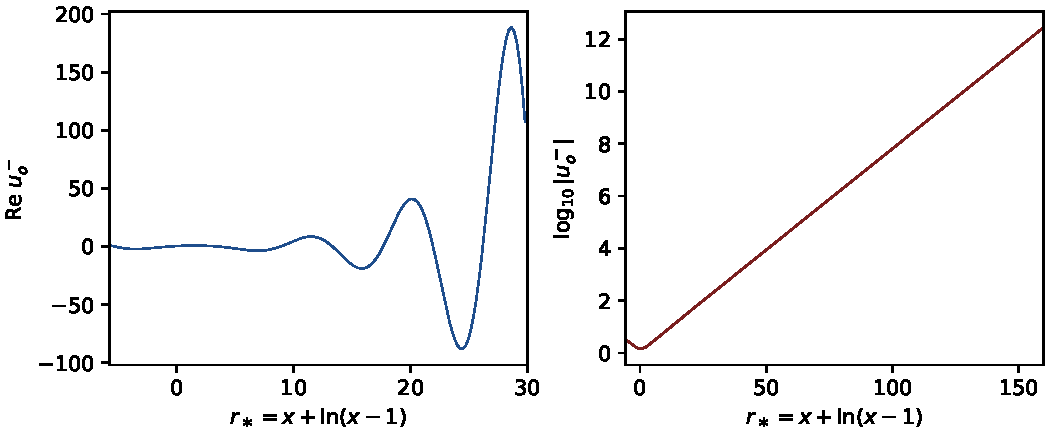
\includegraphics[width=0.98\textwidth]{fig_qnm_curve.pdf}
\caption{Radial profile of the fundamental $\ell=2$ Schwarzschild quasinormal mode,
normalized to unit ingoing amplitude at the horizon, evaluated by one planned transport
with shared-coefficient buckets at requested relative accuracy $10^{-10}$. Left: real part
of the master function $u^{-}_{o}(x)$ in the near-barrier window $r_\ast\le30$, where it
stays at natural scale. Right: $\log_{10}|u^{-}_{o}|$ across the full truncated domain;
the magnitude spans twelve decades between the barrier region and the truncated outer
end.}
\label{fig:qnm-curve}
\end{figure}

\section{Verification against independent references}
\label{sec:verification}

Three layers of verification accompany the package. First, the shipped examples are
self-checking: every script compares its output against a closed form, an independently
implemented recurrence, or a counterfactual control before reporting success, as in
section~\ref{sec:examples}. Second, the Python and Wolfram test suites (181 unit tests
and 26 end-to-end Wolfram checks) run the public interfaces against internal consistency
requirements---round trips of every serialized format, rejection of malformed input,
plan/execute separation, precision gates, save-point contracts and the exact-gate
behavior of section~\ref{sec:certification}---and were re-executed fresh for this paper.
Third, independent validation directories exercise the released tree from empty result
folders: a 16-dimensional exact system over $\mathbb Q(\ii)(k)$ cross-checks complete
endpoint vectors between the package and a separately written driver, and the singular
target classification is validated on translated targets (for example $2+\ii$ beside
$5+\ii$) so that the classification cannot degenerate to a special-cased letter or
coordinate. The package does not ship a timing benchmark against other programs, and no
relative performance claim is made here.

\section{Summary and outlook}
\label{sec:summary}

\texttt{FlintNDE} provides a fast, plain numerical solver for first-order matrix
differential equations with rational or analytic coefficients, built on FLINT ball
arithmetic so that every result carries a rigorous error estimate. Its certified workflow
runs from exact structural input through generalized power series, adaptive path planning
with plan/execute separation, and reusable save points to regulator-series
reconstruction, and is exposed from both Python and Wolfram Language. The Schwarzschild
quasinormal-mode example demonstrates that the same contract solves a two-ended radial
connection problem with irregular endpoints, and the remaining examples cover each public
interface.

The supported classes of irregular singularities are deliberately strict: the package
certifies decoupled essential singularities and start-only second-order formal branches, and
fails closed on ramified gauges, algebraic extensions beyond $\mathbb Q(\ii)$, general
formal block decoupling and Stokes connections. Shipping public Feynman-integral examples
with same-input benchmarks against existing programs, and promoting the regulator-neutral
and epsilon-jet modules to top-level interfaces, are natural next steps.

\section*{Acknowledgments}

Jiaqi Chen is supported by the National Natural Science Foundation of China (NSFC) under
Grant No.~12505094 and by the Science Foundation of China University of Petroleum, Beijing
(No.~2462025YJRC019).

\medskip
\noindent\textbf{Statement on AI Use.}
The author designed the package notation, user-facing functions and input formats, and set
the overall direction of the implementation. Several agent programs, each driven by a
different large language model, implemented the package and its documentation under the
author's guidance. The validation combines comparisons with independent references and
cross-language consistency checks with internal certification gates.

\noindent The package is available at \url{https://github.com/J7C/dSIBP-Packages}.

\appendix

\section{Public interface}
\label{app:api}

The Python package exports its stable interface through \texttt{flintnde.\_\_all\_\_};
four modules (\texttt{regular\_point\_de}, \texttt{epsilon\_jet\_de},
\texttt{mathematica\_bridge}, \texttt{savepoints}) are public at module level only. The
Wolfram interface exports the symbols of section~\ref{sec:wolfram}.

\begin{table}[!ht]
\centering
\footnotesize
\caption{Public interface by layer.}
\label{tab:api}
\begin{tabular}{@{}l>{\raggedright\arraybackslash}p{0.70\textwidth}@{}}
\toprule
Layer & Exported names\\
\midrule
Numerics & \texttt{DEFAULT\_WORKING\_PRECISION\_DIGITS},
\texttt{FLINTNDE\_CITATION\_NOTICE}, \texttt{configure\_working\_precision},
\texttt{acb\_midpoint\_matrix},
\texttt{column\_vector}, \texttt{vector\_norm\_inf},
\texttt{relative\_difference\_inf}\\
Exact input & \texttt{GaussianRational}, \texttt{gaussian\_rational},
\texttt{rational\_function}\\
Systems & \texttt{RationalMatrixSystem}, \texttt{RationalFunction},
\texttt{analyze\_singularities}, \texttt{SingularityInventory},
\texttt{SingularityRecord}, \texttt{AnalyticMatrixSystem},
\texttt{PartialFractionSystem}\\
Local bases & \texttt{RegularSingularSystem}, \texttt{build\_frobenius\_manifest},
\texttt{build\_exact\_frobenius\_manifest}, \texttt{build\_power\_log\_basis},
\texttt{PowerLogBasis}, \texttt{NumericalRegularSingularSystem},
\texttt{NumericalFrobeniusOptions},
\texttt{build\_numerical\_frobenius\_manifest}, \texttt{build\_local\_solution\_basis},
\texttt{LocalSolutionBasis}, \texttt{LocalReductionError},
\texttt{attempt\_fuchsian\_reduction}, \texttt{MoserBalanceTransformation},
\texttt{FuchsianReductionResult}\\
Boundaries & \texttt{frobenius\_boundary}, \texttt{FrobeniusBoundary},
\texttt{FrobeniusBoundaryTerm}, \texttt{exponential\_boundary},
\texttt{ExponentialBoundary}, \texttt{ExponentialBoundaryTerm}\\
Routing & \texttt{NamedPoint}, \texttt{classify\_point}, \texttt{PointClassification},
\texttt{prepare\_local\_expansion}, \texttt{LocalExpansion},
\texttt{build\_adaptive\_path}, \texttt{build\_adaptive\_path\_plan}, \texttt{PathPlan},
\texttt{AdaptivePath}, \texttt{AdaptivePathSingularityError},
\texttt{adaptive\_path\_to\_json}, \texttt{adaptive\_path\_from\_json},
\texttt{plan\_transport\_path}, \texttt{direct\_user\_point\_path},
\texttt{transport\_planned\_path}, \texttt{transport\_planned\_path\_refined},
\texttt{PlannedPath}, \texttt{SingularityJumpSpec}, \texttt{SingularityJumpBasis},
\texttt{SingularityJumpError}, \texttt{SingularPathError},
\texttt{planned\_path\_to\_json}, \texttt{planned\_path\_from\_json}\\
Singular targets & \texttt{plan\_singular\_target\_match},
\texttt{evaluate\_singular\_target}, \texttt{SingularTargetResult},
\texttt{SingularTargetMatchPlan}\\
Transport & \texttt{build\_straight\_path}, \texttt{transport\_path},
\texttt{transport\_path\_refined}, \texttt{transport\_frobenius\_boundaries\_refined}\\
Reconstruction & \texttt{reconstruct\_series\_solution},
\texttt{SeriesReconstructionResult}, \texttt{SeriesValidationError},
\texttt{fit\_sampled\_series}\\
Parallelism & \texttt{run\_ep\_tasks}, \texttt{EpTaskBatchResult},
\texttt{DEFAULT\_PARALLEL\_TASK\_COUNT}\\
Diagnostics & \texttt{five\_term\_tail\_diagnostic},
\texttt{FiveTermTailDiagnostic}\\
Output & \texttt{initialize\_output\_layout}, \texttt{OutputLayout}\\
Wolfram & \texttt{\$FlintNDEVersion}, \texttt{FlintNDERationalSystem},
\texttt{FlintNDEPartialFractionSystem}, \texttt{FlintNDEPlanPath},
\texttt{FlintNDEExecutePath}, \texttt{FlintNDEEvaluateEpBatch},
\texttt{FlintNDEBridgeError}\\
\bottomrule
\end{tabular}
\end{table}

\section{Exact arithmetic, thresholds and serialized formats}
\label{app:exact}

The exact backend represents Gaussian rationals as pairs of FLINT \texttt{fmpq} and
complex matrices as pairs of \texttt{fmpq\_mat} of unchanged dimension, with square-free
factorization, characteristic polynomials, nullspaces and reduced row echelon forms
implemented over $\mathbb Q(\ii)$; no external computer algebra system is required for the
certified routes. The numerical structure classification of section~\ref{sec:certification}
uses the relative cutoff
\begin{equation}
  \tau_{\rm rel}=N\,10^{-p},\qquad
  \tau_{\rm abs}=\tau_{\rm rel}\max\!\left(\max_{i,j}|R_{ij}|,\max_{m,i,j}|(A_m)_{ij}|\right),
  \label{eq:numerical-log-threshold}
\end{equation}
where $N$ is the system dimension and $p$ is the reliable decimal precision of the input,
not of the arithmetic. The classification records its full provenance: input precision,
both cutoffs, the matrix scale, and the largest zeroed and smallest retained quantities,
with undefined relative ratios reported as null rather than fabricated.

All serialized records---paths, plans, inventories, local manifests, save points and
reconstruction results---carry versioned schema names (for example
\texttt{flintnde\_adaptive\_path\_plan\_v1},
\texttt{flintnde\_exponential\_power\_log\_v1},
\texttt{flintnde\_series\_reconstruction\_v1}) and are validated with a strict
exact-keys gate: a record with a missing or unexpected field is rejected with a message
that names the expected key set. Ball values serialize as midpoint, radius and exponent,
and plans record their \texttt{planning\_precision\_digits}, which
section~\ref{sec:paths} elevates to an execution gate. Results are laid out in fixed
categories (\texttt{configuration}, \texttt{singularities}, \texttt{frobenius},
\texttt{transport}, \texttt{regularization}, \texttt{summary}) beside the calling script,
never inside the package source tree.

\bibliographystyle{JHEP}
\bibliography{references}

\end{document}
